%%% Einfaches Template für einen Abschlussbericht zum Berufspraktikum
%%% äöüÄÖÜß  <-- keine deutschen Umlaute hier? UTF-faehigen Editor verwenden!

%%% Magic Comments zum Setzen der korrekten Parameter in kompatiblen IDEs
% !TeX encoding = utf8
% !TeX program = pdflatex 
% !TeX spellcheck = de_DE
% !BIB program = biber

\RequirePackage[utf8]{inputenc} % bei Verw. von lualatex oder xelatex entfernen!
\RequirePackage{hgbpdfa}        % Erzeugt ein PDF/A-2b-konformes Dokument

\documentclass[internship,german,smartquotes,alphabetic]{hgbthesis}
% Zulässige Optionen in [..]: 
%    Typ der Arbeit: 'diploma', 'master' (default), 'bachelor', 'internship'
%		 Zusätzlich für ein Thesis-Exposé: 'proposal' (für 'bachelor' und 'master')
%    Hauptsprache: 'german' (default), 'english'
%    Option zur Umwandlung in typografische Anführungszeichen: 'smartquotes'
%    APA Zitierstil: 'apa'
%%%-----------------------------------------------------------------------------

\graphicspath{{images/}}  % Verzeichnis mit Bildern und Grafiken
\logofile{logo}           % Logo-Datei: images/logo.pdf (kein Logo: \logofile{})
\bibliography{references} % Biblatex-Literaturdatei (references.bib)

\usepackage{hyperref}
\usepackage[acronym]{glossaries}

\makeglossaries

\newacronym{jvm}{JVM}{Java Virtual Machine}
\newacronym{vt}{VT}{Virtual Thread}
\newacronym{pt}{PT}{Plattform Thread}
\newacronym{ot}{OT}{Betriebssystem Thread}
\newacronym{sts}{STS}{StructuredTaskScope}                          % makeglossaries main in der cmd ausführen
\makeglossaries                           % makeglossaries muss dadurch nicht mehr in der cmd ausgeführt werden  

%%%-----------------------------------------------------------------------------
\begin{document}
%%%-----------------------------------------------------------------------------

%%%-----------------------------------------------------------------------------
% Angaben für die Titelei (Titelseite, Erklärung etc.)
%%%-----------------------------------------------------------------------------

% \title{Endbericht zum Berufspraktikum bei Mogulovich International}
% \author{Alex A.\ Schlaumeier}

% \programtype{Fachhochschul-Bachelorstudiengang}
% \programname{Medientechnik und -design}
% \placeofstudy{Hagenberg}

% \dateofsubmission{2024}{06}{25}
% \advisor{Pjotr I.~Czar, M.A.}
% \companyName{%
%    Mogulovich International Media GmbH\\
%    Online Division\\
%    Hubertusgasse 3a, 1020 Wien
% }
% \companyUrl{www.mogul.at}
\pagenumbering{alph}                    % damit die Titelseite mit 'a' beginnt und links wieder richtig funktionieren
% 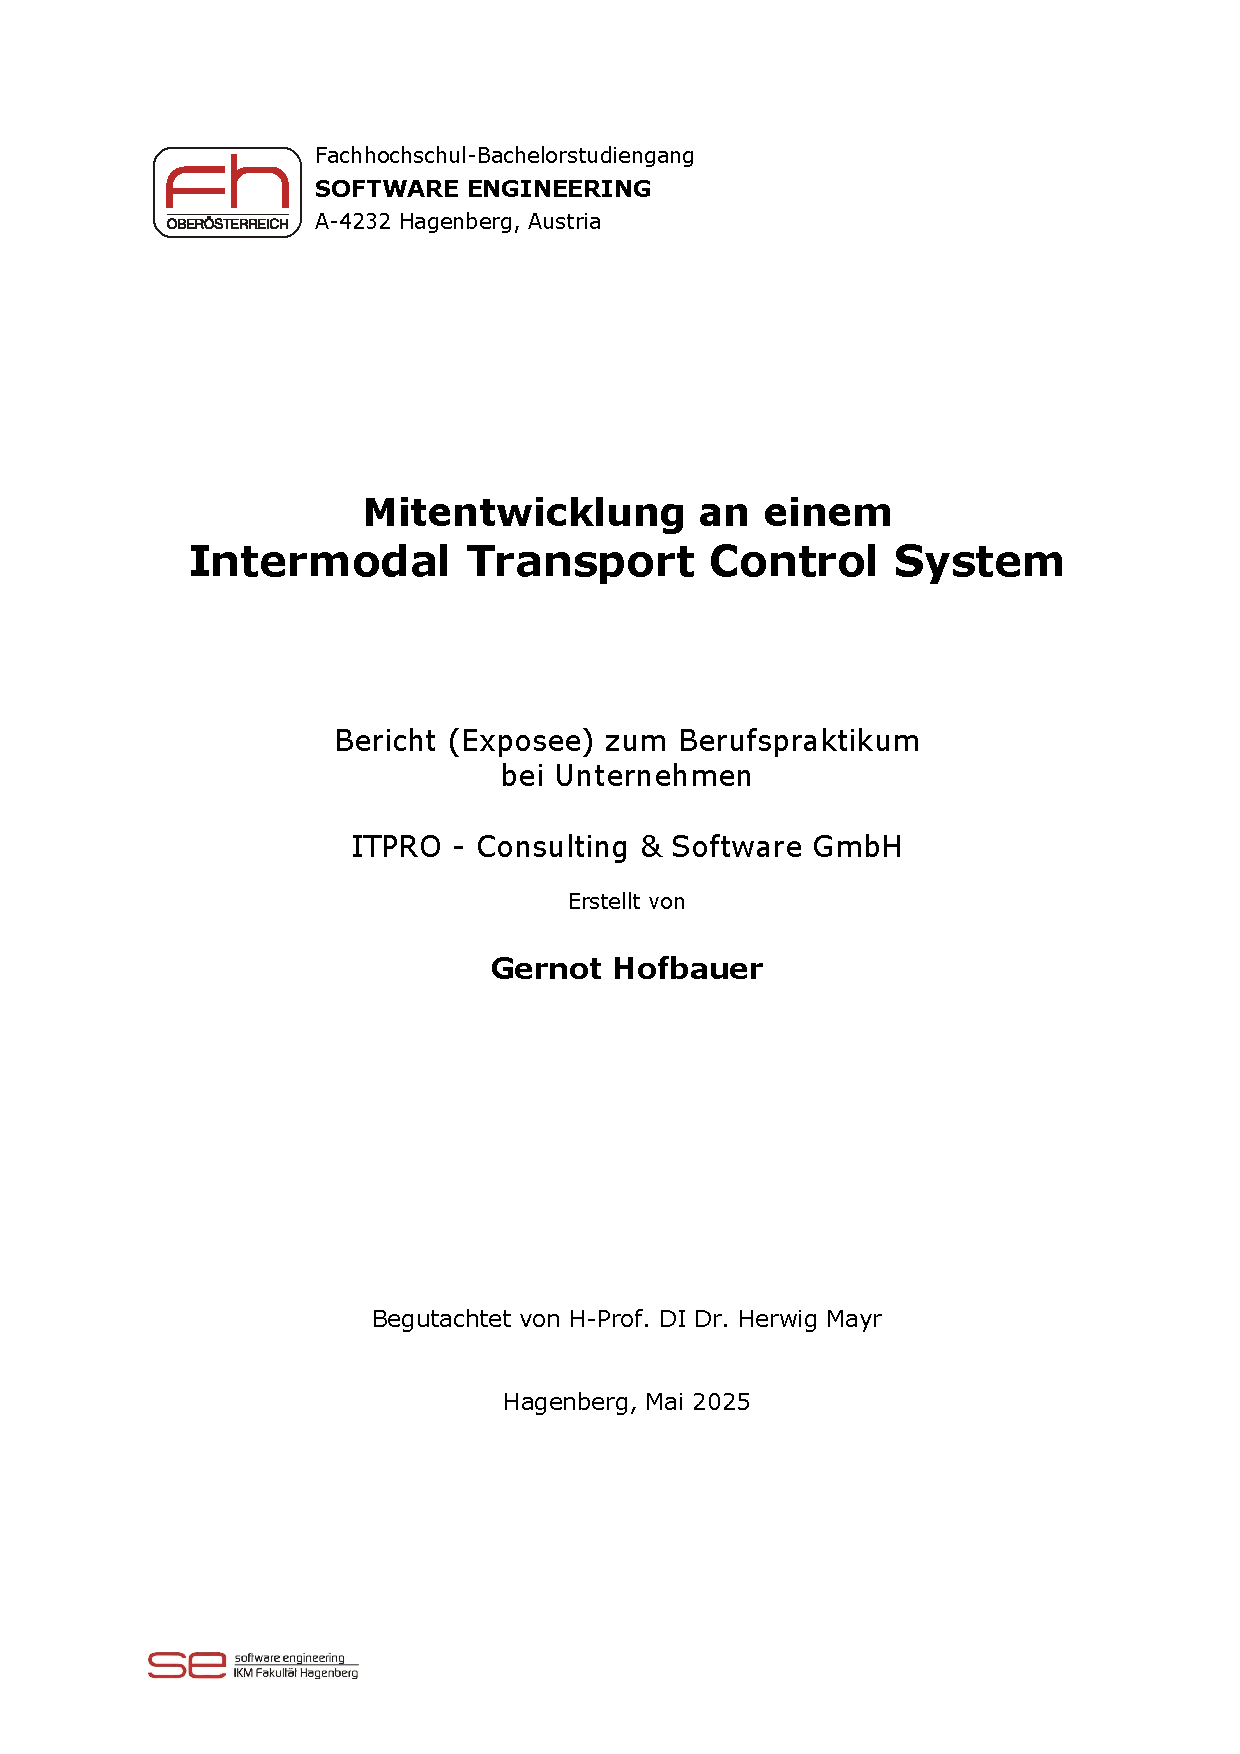
\includepdf[pages=-]{Titelblatt.pdf}
%%%-----------------------------------------------------------------------------
\frontmatter                                       % Titelei (röm. Seitenzahlen)
%%%-----------------------------------------------------------------------------

% \maketitle
\tableofcontents
\printglossary[type=\acronymtype,title=Akronyme]

%%%-----------------------------------------------------------------------------

\chapter{Kurzfassung}% Umfang der Kurzfassung: ca.\ 200 Worte.
Dieser Praktikumsbericht beschreibt die Arbeit des Praktikanten im Rahmen seines Praktikums bei der Firma ITCS GmbH. Der Schwerpunkt lag auf der Entwicklung
von Software für das ITCS-Management-System, das in der öffentlichen Verkehrsinfrastruktur eingesetzt wird. Das Herzstück dieser Software ist eine Webanwendung,
die es ermöglicht, Umläufe aus einzelnen Fahrten zu erstellen. Dabei sollten verschiedene benötigte Daten auf der darunterliegenden Datenbank generiert werden.
Außerdem sollten diese Umläufe auch automatisch auf Durchführbarkeit geprüft werden.
In diesem Praktikum wurde mit der Programmiersprache \emph{C\#} und dem \emph{.NET}-Framework gearbeitet. Der Datenbankzugriff erfolgte über die \emph{Entity Framework Core}-Bibliothek, 
die eine objektorientierte Abstraktionsebene für den Datenbankzugriff bereitstellt. Das Frontend wurde mit \emph{Blazor} entwickelt, einer modernen Webtechnologie, 
die es ermöglicht, interaktive Webanwendungen mit C\# zu erstellen. Durch die Verwendung von \emph{Blazor} konnte eine nahtlose Integration zwischen Frontend und Backend erreicht werden,
was die Entwicklung effizienter und flexibler machte.
Während der Implementierung diese Umlaufeditors musste auch teilweise das bestehende Datenmodell angepasst werden, um die neuen Anforderungen zu erfüllen. 
Da die Datenbank mit Daten aus anderen Systemen gefüllt wird, musste auch ein anderes, bestehendes Projekt, das für den Import und Export von Daten benutzt ist, angepasst werden.
Dabei musste darauf geachtet werden, dass die Daten weiterhin mit dem \emph{VDV-452}-Standard kompatibel bleiben, um die Interoperabilität mit anderen Systemen zu gewährleisten.

%%%-----------------------------------------------------------------------------
\mainmatter                             % Hauptteil (ab hier arab. Seitenzahlen)
%%%-----------------------------------------------------------------------------
\chapter{Einleitung}
\label{cha:Einleitung}

    Seit einigen Jahren Arbeitet Oracle an Möglichkeiten zur Verbesserung der Skalierbarkeit von Java-Anwendungen im Projekt "Loom".
    Der Hauptansatz dieses Vorhabens ist die Einführung von virtuellen Threads, die von der JVM verwaltet werden. 
    Diese Threads sind leichtgewichtiger als klassische Plattform Threads und können in größerer Anzahl erzeugt werden.
    So können bestimmte Anwendungen mit hoher Nebenläufigkeit zukünftig effizienter gestaltet werden. Diese Bachelorarbeit 
    beleuchtet diese Technologien und stellt die Neuerungen dem bereits Bekanntem gegenüber.

\section{Ziel der Arbeit}
\label{sec:Ziel}

    Das Ziel dieser Bachelorarbeit ist es, die grundlegenden Eigenschaften und Limitierungen des bestehenden Thread-Konzepts zu untersuchen und die Motivationen für die Neuerungen
    durch Projekt Loom zu verstehen. Ein Überblick über Projekt Loom und die damit verbundenen Technologien wird gegeben, wobei der Schwerpunkt auf Virtual Threads liegt. 
    Die Arbeit soll zeigen, wie und in welchen Fällen diese Neuerungen in der Praxis angewendet werden können und welche neuen Möglichkeiten sich dadurch ergeben. 
    Es wird auch verdeutlicht, welche bestehenden Probleme der parallelen Ausführung durch die neuen Technologien nicht gelöst werden können. 
    Durch Benchmarks sollen Laufzeit und Speicherverbrauch unter verschiedenen Umständen analysiert werden, um daraus Schlüsse zu ziehen, 
    in welchen Fällen die neuen Technologien verwendet werden sollten und in welchen nicht. Als konkretes Ergebnis wird eine Sammlung kleinerer Programme erstellt, 
    die die neuen Technologien in Projekt Loom demonstrieren und die Unterschiede zu den bisherigen Technologien aufzeigen.




% \chapter{Das Unternehmen}

% Umfang: 1--2 Seiten
% %%%-----------------------------------------------------------------------------

% \chapter{Projekte und Tätigkeiten während des Praktikums}

% Umfang: 2--3 Seiten (Projektziel(e), Projektumfeld)

% %%%-----------------------------------------------------------------------------
     
% \chapter{Projektbeispiele}

% Umfang: 5--6 Seiten (Umsetzung, grober Terminplan, Ergebnisse,
% Qualitätssicherungsmaßnahmen)

% %%%-----------------------------------------------------------------------------

% \chapter{Erfahrungen und Zusammenfassung}

% Umfang: 1--2 Seiten

%%%-----------------------------------------------------------------------------
%\backmatter        % Schlussteil (nur bei Verwendung des Quellenverzeichnisses)
%%%-----------------------------------------------------------------------------

\MakeBibliography % Quellenverzeichnis (sofern notwendig, sonst weglassen)

\end{document}
